\documentclass[12pt,a4paper]{article}
\usepackage{graphicx}

\begin{document}

\begin{titlepage}

\center{\Huge{The Black Box}}
\center{\large{Human perception in the 19th century}}
\vspace{1cm}

\begin{figure}[h]
	\centering
	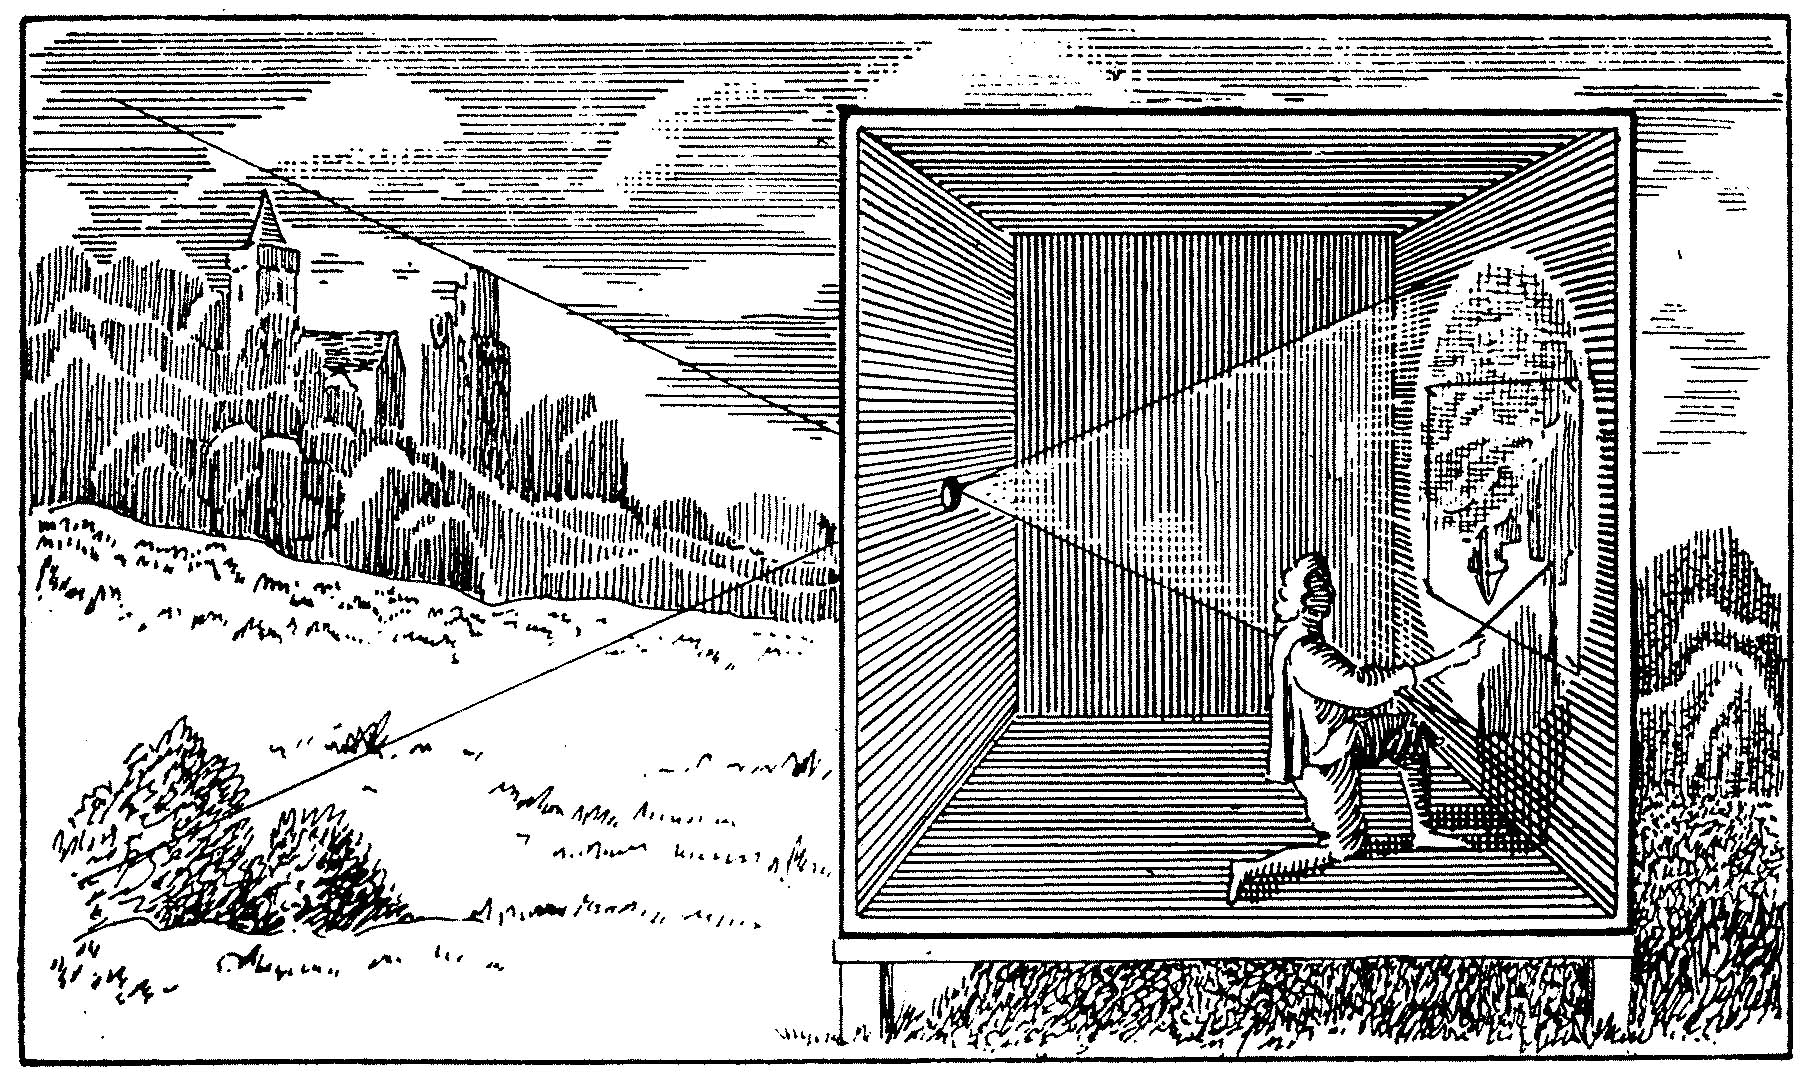
\includegraphics[width=\textwidth]{img/cameraobscura.jpeg}
\end{figure}

\vspace{1cm}
\center{Dominik Schlegel}
\center{\today}

\end{titlepage}


\newpage

\section*{Preface}

On the following pages I will discuss the development of the human perception model and its
inseparable relations to the scientific body in the 19th century. The essay focusses on
{\it{Subjective Vision and the Separation of the Senses}} \cite{crary} and includes information from
{\it{Techniques of the Observer}} \cite{crary}, {\it{The Images of Precision: Helmholtz and the
graphical Method in Physiology}} \cite{holmes} and {\it{Camera and Mind}} \cite{ellenbogen}. Basic
knowledge of the material is assumed and only the key points will be repeated in order to explain
my view.

As an additional source I picked a topic about the beginning of the institutionalization of people
with disabilities during the 19th century and its direct connection to the respective idea of
perception and human society \cite{crary}.

\section*{Thesis}

I claim that the change from the 18th centuries humanly passive and pseudo-objective
perception to the physiologically objective perception of the 19th century was crucial in order to
enable the massive growth in production of scientific knowledge during the 19th century.
The human body was far from being completely understood at the end of the 18th century but
nevertheless people took perceived impressions as the undiluted, completely clear representation of
their true nature.
This premise reduces the observer to a simple, passive receiver of information without any transformation
of the input from outside - which is not entirely true as we know nowadays.
One can easily think about the numerous possible conflicts resulting from parties with differently developed
senses (e.g. eyesight).

At the same time researches started to play around with the senses and challenged this humanly passive model
of perception. As a result people became unsure about the intake of their senses and the human body
manifested itself as the nature of perception (from physics to physiology). The human body can therefore be
seen as a black box, an object in which we do not not what is going on but in which we expect a
transformation of the input. The step to the acceptance of this black box is of prime importance to me.
Having the black box model researchers could start to quantify perception and get closer to truth
representations of nature.

Additionally one should not forget the inherent link between the new model of perception and human society.
The researchers pursuing the new model of perception had many contestants and had a hard time publishing
their findings in the beginning of the physiological movement.

\newpage

Relating to my second source, people whose senses were non- or malfunctional were not able to perceive nature
based on the humanly passive model - and as a consequence were not accepted by the broad human society. This
changed with the model of perception, whereas it became clear that every human transforms nature and
therefore nobody can tell the actual truth of an occurrence. I do not say that this was the major reason for
rise of the institutionalization of people with disabilities but it certainly did play its part.

\section*{Reading}

{\it{Subjective Vision and the Separation of the Senses}} is a chapter of the book {\it{Techniques of the
Observer}} \cite{crary} written by Jonathan Crary. The essay is composed upon a literature collection and
refers to various famous historical figures. The two major topics discussed are the rise of physiology and
the establishment and reframing of new sciences.



\newpage




Ladida I have absolutely no idea what I'm  talking about in this actual current sentence and do not
know how to turn on auto correct for this damn tool assddas.
Test \cite{crary} \cite{holmes} \cite{ellenbogen} \\
This is another Test \\

Test ladiasdas and here we are again \\
Knowingly not knowing \\
Test test test \\

And another section


\newpage

\bibliographystyle{unsrt}
\bibliography{references.bib}

\end{document}
